\section{Recommendation Aggregation}\label{sec:aggregations}
In this section we explain the workings and concept behind the four aggregation methods.

\note{Rewrite this to preprocessing}
Ranking is the idea of the position of an item in a ranked list is important. This means that if there is a list of ratings $\tau$ the list is ranked if $\tau (1) > \tau (2) > ... > \tau (k)$

When we talk about a top-k list in this paper we are referring to an ranked list of user preferences which is ordered by their item ratings in descending order.

There are several reasons for the use of ranked lists. 
The first reason is that we want to return a ranked list as a result of the aggregation since we want to ease the decision-making without making the final decision.
Secondly, there are a good selection of measurements for the quality of a ranked list. Many of these measures take two lists, $\tau_1$ and $\tau_2$, which are both ranked lists of the same size. 

In our case one of the lists is a top-k list and the second list is the ranked list of recommendations.
\adparagraph{Borda Count}
Aside from SF in the SFD measure, and Adjusted nDCG, BC was the best performing method.
\begin{figure}[H]
	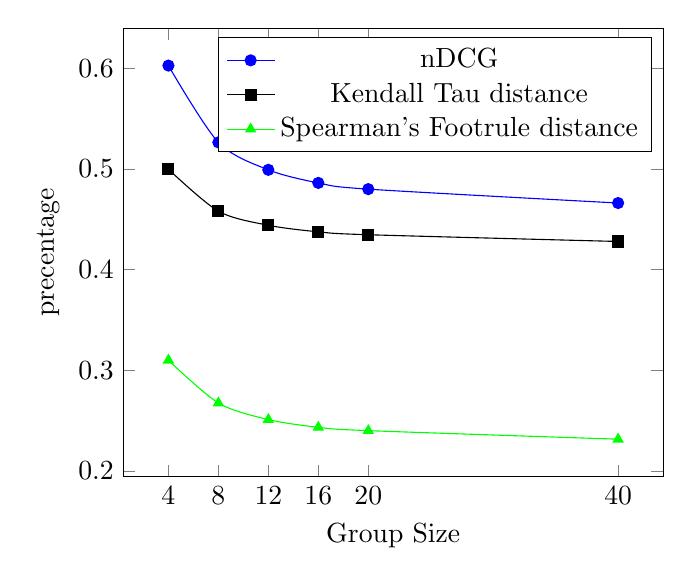
\begin{tikzpicture}
	\begin{axis}[
	xlabel=Group Size,
	ylabel=precentage,
	xtick = {4,8,12,16,20,40}]
	\addplot[smooth,mark=*,blue] plot coordinates {
		(4,0.6028)
		(8,0.5265)
		(12,0.4992)
		(16,0.4862)
		(20,0.48)
		(40,0.4662)
	};
	\addlegendentry{nDCG}
	
		\addplot[smooth,color=black,mark=square*] plot coordinates {
		(4,0.4998)
		(8,0.4581)
		(12,0.4441)
		(16,0.4376)
		(20,0.4347)
		(40,0.428)
	};
	\addlegendentry{Kendall Tau distance}
	
		\addplot[smooth,color=green,mark=triangle*] plot coordinates {
		(4,0.31)
		(8,0.2675)
		(12,0.251)
		(16,0.2433)
		(20,0.24)
		(40,0.2315)
	};
	\addlegendentry{Spearman's Footrule distance}
	
	\end{axis}
	\end{tikzpicture}
	\caption{Results for Borda Count}\label{fig:ndcganalysis}
\end{figure}

\begin{table}[H]
\centering
\label{my-label}
\begin{tabular}{|l|lllll|}\hline
     & 4 to 8 & 8 to 12 & 12 to 16 & 16 to 20 & 20 to 40 \\\hline
nDCG & 12.66  & 5.19    & 2.6      & 1.28     & 2.88     \\
KTD  & 8.34   & 3.06    & 1.46     & 0.66     & 1.54     \\
SFD  & 13.71  & 6.17    & 3.07     & 1.36     & 3.54     \\\hline
\end{tabular}
\caption{Percentage decrease between the groups for Borda Count}
\end{table}
\subsubsection{Markov Chain}\label{sec:markovchain}
%Dwork et al propose a Markov Chain for aggregating ranked lists called \MC\cite{rank:aggregation}. \MC has a set of states, $S = \{1, 2,..., |I|\}$, corresponding to a set of all the items, $I$.

Dwork et al propose a Markov Chain for aggregating ranked lists, called \MC\cite{rank:aggregation}. \MC generalizes the heuristics of the Copeland Method, where a winner is the candidate which wins the most pairwise contests\cite{saari1996}.

\MC is a process where we note the possibility of transitioning from one state to another state over time. The \MC state space, $S$, corresponds to a set of all the items, $I$, such that $S = \{1, 2,..., |I|\}$. The transition probabilities between states are represented by a transition matrix, $P = |I| \times |I|$, covering the probability, $p_{ij}$, between any item pair $i \in I$ and $j \in I$.

To calculate the probabilities, let $c_i$ be the set of items from $I$, that for the majority of the ranked lists we aggregate for, $\tau_1, \tau_2, ...,\tau_u$, it holds that $\tau_u(i) > \tau_u(j)$. The probabilities of $P$ is found according to Equation \ref{eq:markovchain_p_ij}. $\lambda$ is a variable for teleporting, which provides a small increase in accurate. Via tuning, we found that $\lambda = 0.05$ is a good value. For the case of a missing item from either or both lists, the item is considered to be on the lowest possible rank.

\begin{equation}\label{eq:markovchain_p_ij}
p_{ij} = (\frac{|c_i|}{|I|})(1-\lambda)+(\frac{\lambda}{|I|})
\end{equation}

For the probability of state $i$ staying in state $i$, we have Equation \ref{eq:markovchain_p_ii}.

\begin{equation}\label{eq:markovchain_p_ii}
p_{ii} = (\frac{|I|-|c_i|}{|I|})(1-\lambda)+(\frac{\lambda}{|I|})
\end{equation}

When the transition matrix is calculated, the result can be found via the stationary distribution for $P$. A distribution vector is a vector of size $|I|$, which holds non-negative values, representing how the states are distributed. For an initial distribution, $x$, then $xP^t$, is the same initial distribution after $t$ steps down the chain. The stationary distribution is where the state distribution stops changing regardless of taking more steps.

For practical purposes, we can approximate the stationary distribution for $P$ via application of the power-iteration algorithm. So the approximate distribution, $r$, is found in Equation \ref{eq:markovchain_power} for a number of steps, $t$. Via tuning, we found that $t = 30$ was a good value.

\begin{equation}\label{eq:markovchain_power}
r = xP^t
\end{equation}

The result of \MC is then found as the $k$ items with the biggest shares of $r$.
\subsection{Spearman's Footrule}\label{sec:spearmansfootrule}
Dwark et al also propose to use Spearman's footrule(SF) for aggregating ranked lists\citep{rank:aggregation}.
SF utilises the graph theory called bipartite graphs to construct a weighted complete bipartite graph $(S,P,W)$. 
Let $S$ be the set of items which is equal to the union of the ranked top-k lists $\tau_1, ..., \tau_k$. Then we have the set $P = \{1,...,k\}$ which is the available positions. Lastly the set $W$ is the set of edge weights between items $s\in S$ and positions $p\in P$. The weights $W(s,p)$ is found by using the scaled footrule distance equation which can be seen in equation \ref{eq:spearmanfootrule}. 
 
%$I$ is the union of users top-k lists and $P$ is the total number of positions equal to $|I|$. $E$ is the weight between an item $i \in I$ and a position $p \in P$. In Equation \ref{eq:spearmanfootrule} it is shown how the weights are calculated for full lists. 

%where the weight on the edges in $E$ is the footrule distance from note u to position v. utilises the minimum cost maximum matching method to find the best possible ranked list based on a set $L$ of ranked lists. 

\begin{equation}\label{eq:spearmanfootrule}
W(c,p) = \displaystyle\sum_{i=1}^{k} |r_i(c)/|r_i| - p/k|
\end{equation}

As we work with partial lists we will encounter lists with missing items. For this reason we have added a second case, in addition to the approach described by Dwark et al, which can be seen in Equation \ref{eq:spearmanfootruleempty}. In this case we adapt the Spearman's footrule distance variable $\ell$ which is used on partial lists. $\ell$ needs to be larger than $k$ and in our case it is $k + 1$. The reason for this is to punish infrequent items by giving them a higher weight.

\begin{equation}\label{eq:spearmanfootruleempty}
W(c,p) = \displaystyle\sum_{i=1}^{k} |(\ell/|r_i| - p/k|
\end{equation}

After determining the edge weights, the problem can be solved as a minimum cost maximum matching problem, which is the problem of finding the highest number of node matches with the lowest edge cost. To do this, we decided to use the Hungarian method\note{Or an extension called Munkres (sæt en cite)}. The result of this method is the top-k list to be recommended.
\subsection{Average}\label{sec:average}